\itemhead{p.103 练习 · 第3题（教材p.103）}{XJ-B1-C04-PR-P103-Y1370}
\label{XJ-B1-C04-PR-P103-Y1370}
{\footnotesize 湘教版教材p.103 / PDF第110页 / p.103 练习 / 第3题}
\field{原题}{已知幂函数 $f(x)=x^\alpha$ 的图象经过点 $\left(3,\dfrac19\right)$，求这个函数的表达式，并画出它的图象的草图，讨论它的奇偶性和单调性。}
\field{参考答案}{$f(x)=x^{-2}=1/x^2$，定义域 $\mathbb R\setminus\{0\}$，偶函数；在 $(-\infty,0)$ 递增、$(0,+\infty)$ 递减，图象在第一、二象限，经过 $(\pm1,1)$，以坐标轴为渐近方向。}
\begin{center}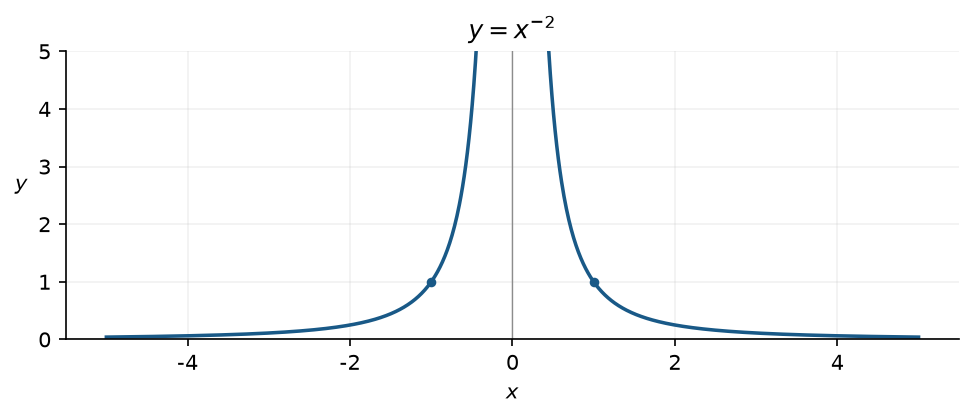
\includegraphics[width=.84\linewidth,height=.38\textheight,keepaspectratio]{figures/C04-PR103-3.png}\end{center}
{\small \field{关联知识}{P03 幂函数的概念、图象与性质（教材帮p.125、126、127 / PDF134、135、136）；F08 奇偶性、对称与函数性质应用（教材帮p.113、114、115 / PDF122、123、124）；F05 单调性定义、证明与参数（教材帮p.97、98、100 / PDF106、107、109）}
\field{方法与易错点}{设 $f(x)=x^\alpha$，用已知点求指数，再查该指数的定义域、奇偶性和各单调区间。 易错：把 $3x^2$ 当标准幂函数；将第一象限性质直接用于负半轴；分数负指数遗漏0禁点。}
\field{答案依据}{答案册相关题组：PDF第30、31页（册内页29、30）；按当前题库原题逐项重算，不按旧版题号机械对套。}}
